
\section{Motivation}

The rapid growth of data generated by large-scale information systems leads to new opportunities for  society and businesses. 
By the end of 2020, the total amount generated data is estimated to be 44 trillion gigabytes, of which 90\% has been created in the last two years \cite{datagrowth}.
In order to benefit from the massive amount of data, efficient solutions are required, that are able to extract potential value in form of models, analyses or predictions.

A remarkable subset of this data is described as \textit{event data}, which is generated by \textit{process-aware information systems}, which manage, execute and monitor business processes \cite{DBLP:journals/topnoc/Aalst09}.
With the non stopping rise of digitization of business processes, increasingly more event data becomes utilizable, thus the potential value of this data is exploding.

The scientific engagement aiming to discover, analyze and improve real processes based on event data led to \textit{process mining}. Process mining bridges the gab between the data-driven characteristic of data science and the process-centric view of process science \cite{DBLP:books/sp/Aalst16}.
The ongoing success of progress mining in research has been transferred to businesses, that successfully offer or utilize this technology.
Celonis, which is often considered as one of the biggest commercial providers of process mining, has been valued 2.5 billion dollar only 9 years after the company was founded \cite{celonis}.

Modern process mining software tends to focus on continuous monitoring and analysis of business processes, in contrast to traditional offline and project-based approaches, that are not integrated with the remaining IT infrastructure of a company.
The integrated and continuous application of process mining is realized by a \textit{business process monitoring system}, which are a key success factor for many organizations, since they allow to understand and supervise all processes of a company in real-time during the execution of the processes.
The core idea of this approach is to automate process mining and keep a persistent data connecting between the information system and the monitoring system, that provides the analytical capabilities.
Figure \ref{fig:process-monitoring} visualizes such an infrastructure and the connection between the systems and the internal and external process stakeholders.

\begin{figure}[htbp!]
	\centering
	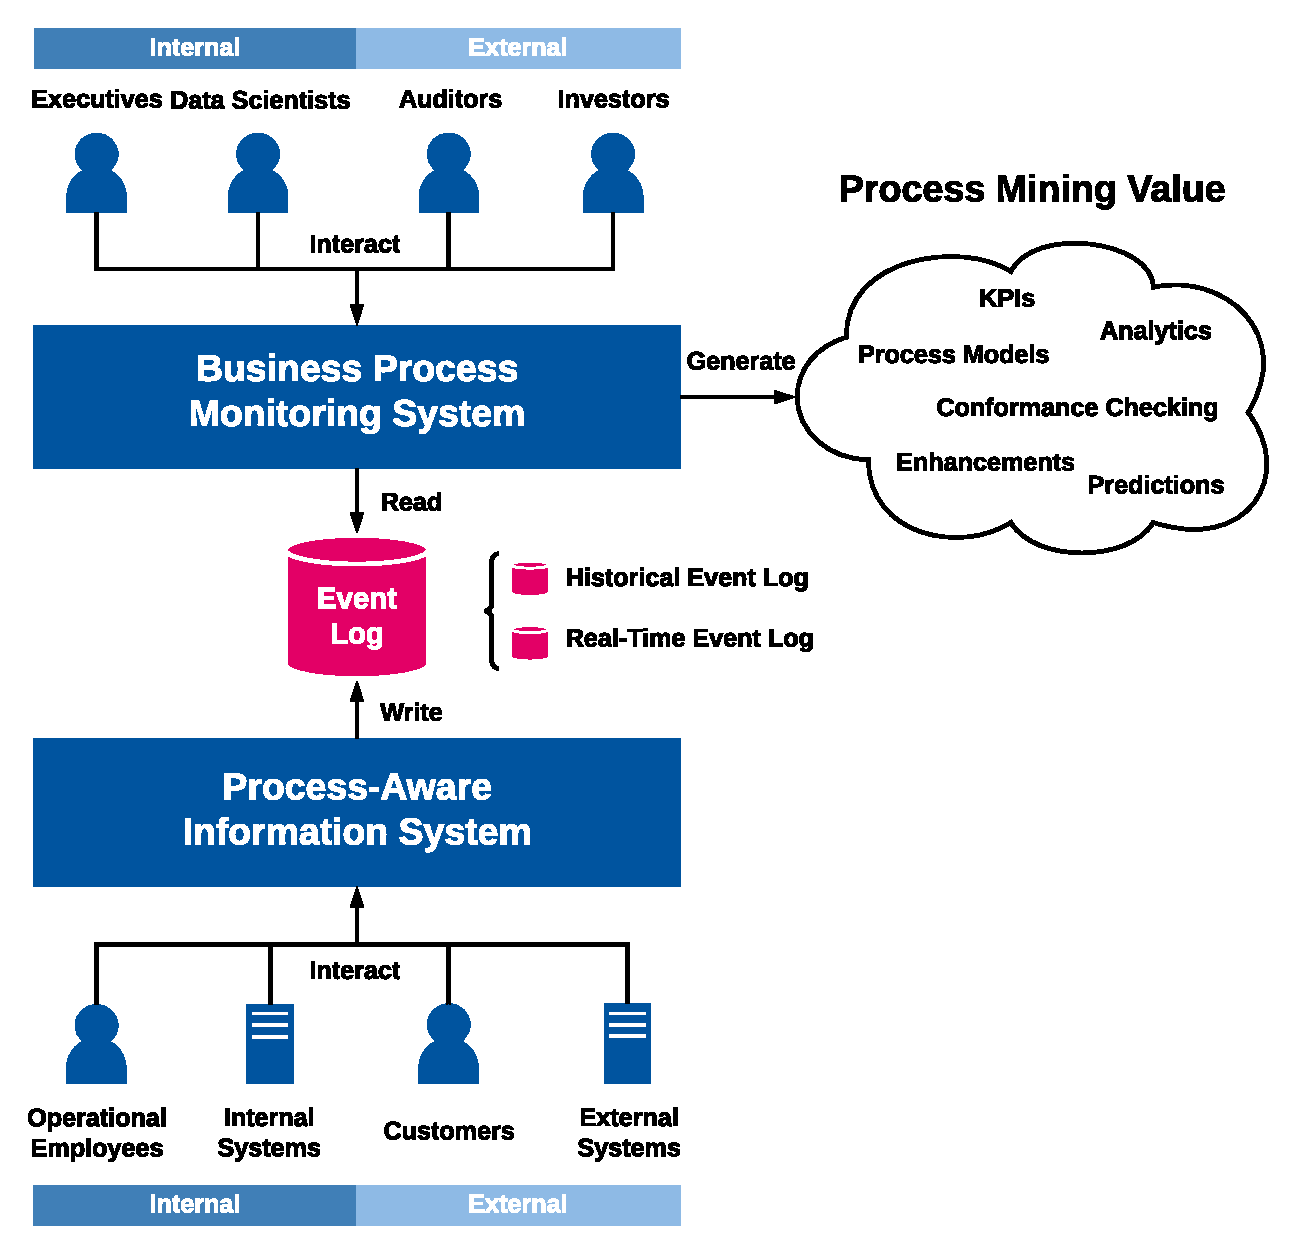
\includegraphics[width=\textwidth]{figures/process-monitoring}
	\caption{Business process monitoring allows to continuously apply process mining techniques in an automated fashion in order to generate value for internal and external process stakeholders.}
	\label{fig:process-monitoring}
\end{figure}

Traditional process mining tends to be backward-looking \cite{DBLP:conf/scsc/Aalst18}, i.e. the focus relies on analyzing and understanding past executions of a process rather than providing value for running process instances in form of predictions or recommendations.
Businesses can develop a competitive advantage, if their process mining solution offers predictive capabilities, that allow to predict the future of a running process instance.
For example, if it is known beforehand, that a running process instance will probably exceed its deadline, measures can be initiated before damage occurs.
Therefore, including the forward-perspective is crucial for a competitive process mining software, especially in the context of business process monitoring.

\section{Problem Statement}

Although, many approaches for process prediction have been suggested in the literature (see Chapter \ref{chap:related_work}), current solutions are limited regarding the data they are able to consider and the targets they predict.
Many approaches derive the prediction purely from the control flow of process instance ignoring additional data attributes in the event log.
Especially, almost no approach is able to consider textual data for process prediction.
In addition, most of the prediction methods focus on a single prediction dimension only, for example they just predict the remaining time until a process instance is finished.
But depending on the context also information about the next event or the future path of process instance can be of interest.
In some scenarios, processes instances have an outcome like success/failure or accepted/declined that can be predicted.

Precisely, given an event log with past executions of a process and a running (i.e. not completed) process instance, we would like to answer the following questions:

\begin{itemize}
	\item What will happen next?
	\item When will it happen?
	\item What is the most likely future path of the instance?
	\item When will the instance finish?
	\item What is the outcome of the instance?
\end{itemize}



\section{Research Goals and Questions}

This thesis aims to improve current state-of-art approaches for process prediction in order to extend the capabilities of process monitoring software.
The main research goal is to design, implement and evaluate a predictive model for event data that is able to take advantage of additional textual data associated with each event.
Since most current approach are not able to handle textual data, we would like to know to what extend textual data can improve the quality of process prediction.
Furthermore, we want to evaluate different design choices and text models for text-aware process prediction and discuss potential trade-offs.

These goals lead to the formulation of the following research questions:

\begin{itemize}
	\item[] \textbf{RQ1} To what extend can the utilization of textual data improve the performance of process prediction?
	\item[] \textbf{RQ2} How does the choice of the text model and other parameters influence the prediction results?
	\item[] \textbf{RQ3} What are the advantages and disadvantages of the approach compared to existing methods?
\end{itemize}

\section{Contribution}



\section{Thesis Structure}

This thesis is structured in seven chapters.
In Chapter \ref{chap:prelim} the notations, definitions and concepts used in this contribution are introduced.
This includes an introduction to process mining, text mining, supervised learning and LSTM neural networks.
Chapter \ref{chap:related_work} summarizes relevant scientific contributions which focus on the problem of prediction in process mining and gives an overview of already available methods and their capabilities.
In Chapter \ref{chap:concept} the novel text-aware process prediction model as main conceptional contribution is presented.
Moreover, Chapter \ref{chap:impl} covers the implementation details of the model on a technical level.
In Chapter \ref{chap:eval} the performance of the new approach is evaluated and compared to current state-of-the-art prediction methods.
Finally, in Chapter \ref{chap:conclusion} the conclusion is given by wrapping up the key results as well as discussing the limitations of the approach.
Furthermore, an outlook towards future potential research questions on process prediction in the context of business process monitoring is given.